\chapter{Review of Circuit QED \label{ch:3_cQED}}

Circuit quantum electrodynamics (cQED) can be described as the study of light-matter interaction in engineered quantum systems built from superconducting circuits. Namely, it deals with nonlinear superconducting \textit{qubits} that act as artificial atoms and which couple to quantized electromagnetic fields in the microwave frequency domain \cite{blais2004cavity}. Over the last 20 years, cQED has become a leading hardware platform for the development of quantum information processing technology \cite{devoret2004superconducting, devoret2013superconducting, girvin2014circuit, krantz2019quantum, kjaergaard2020superconducting, blais2020quantum, blais2021circuit}. In this chapter, we aim to give a brief overview of circuit QED and will specifically discuss three important superconducting circuits: the LC resonator, the transmon qubit, and the fluxonium qubit. Finally, we will dive deeper into the fluxonium and its coupling to a resonator (which will motivate our experimental design in Ch. \ref{ch:4_3DGKP}). 


\begin{figure}[h]
    \centering
    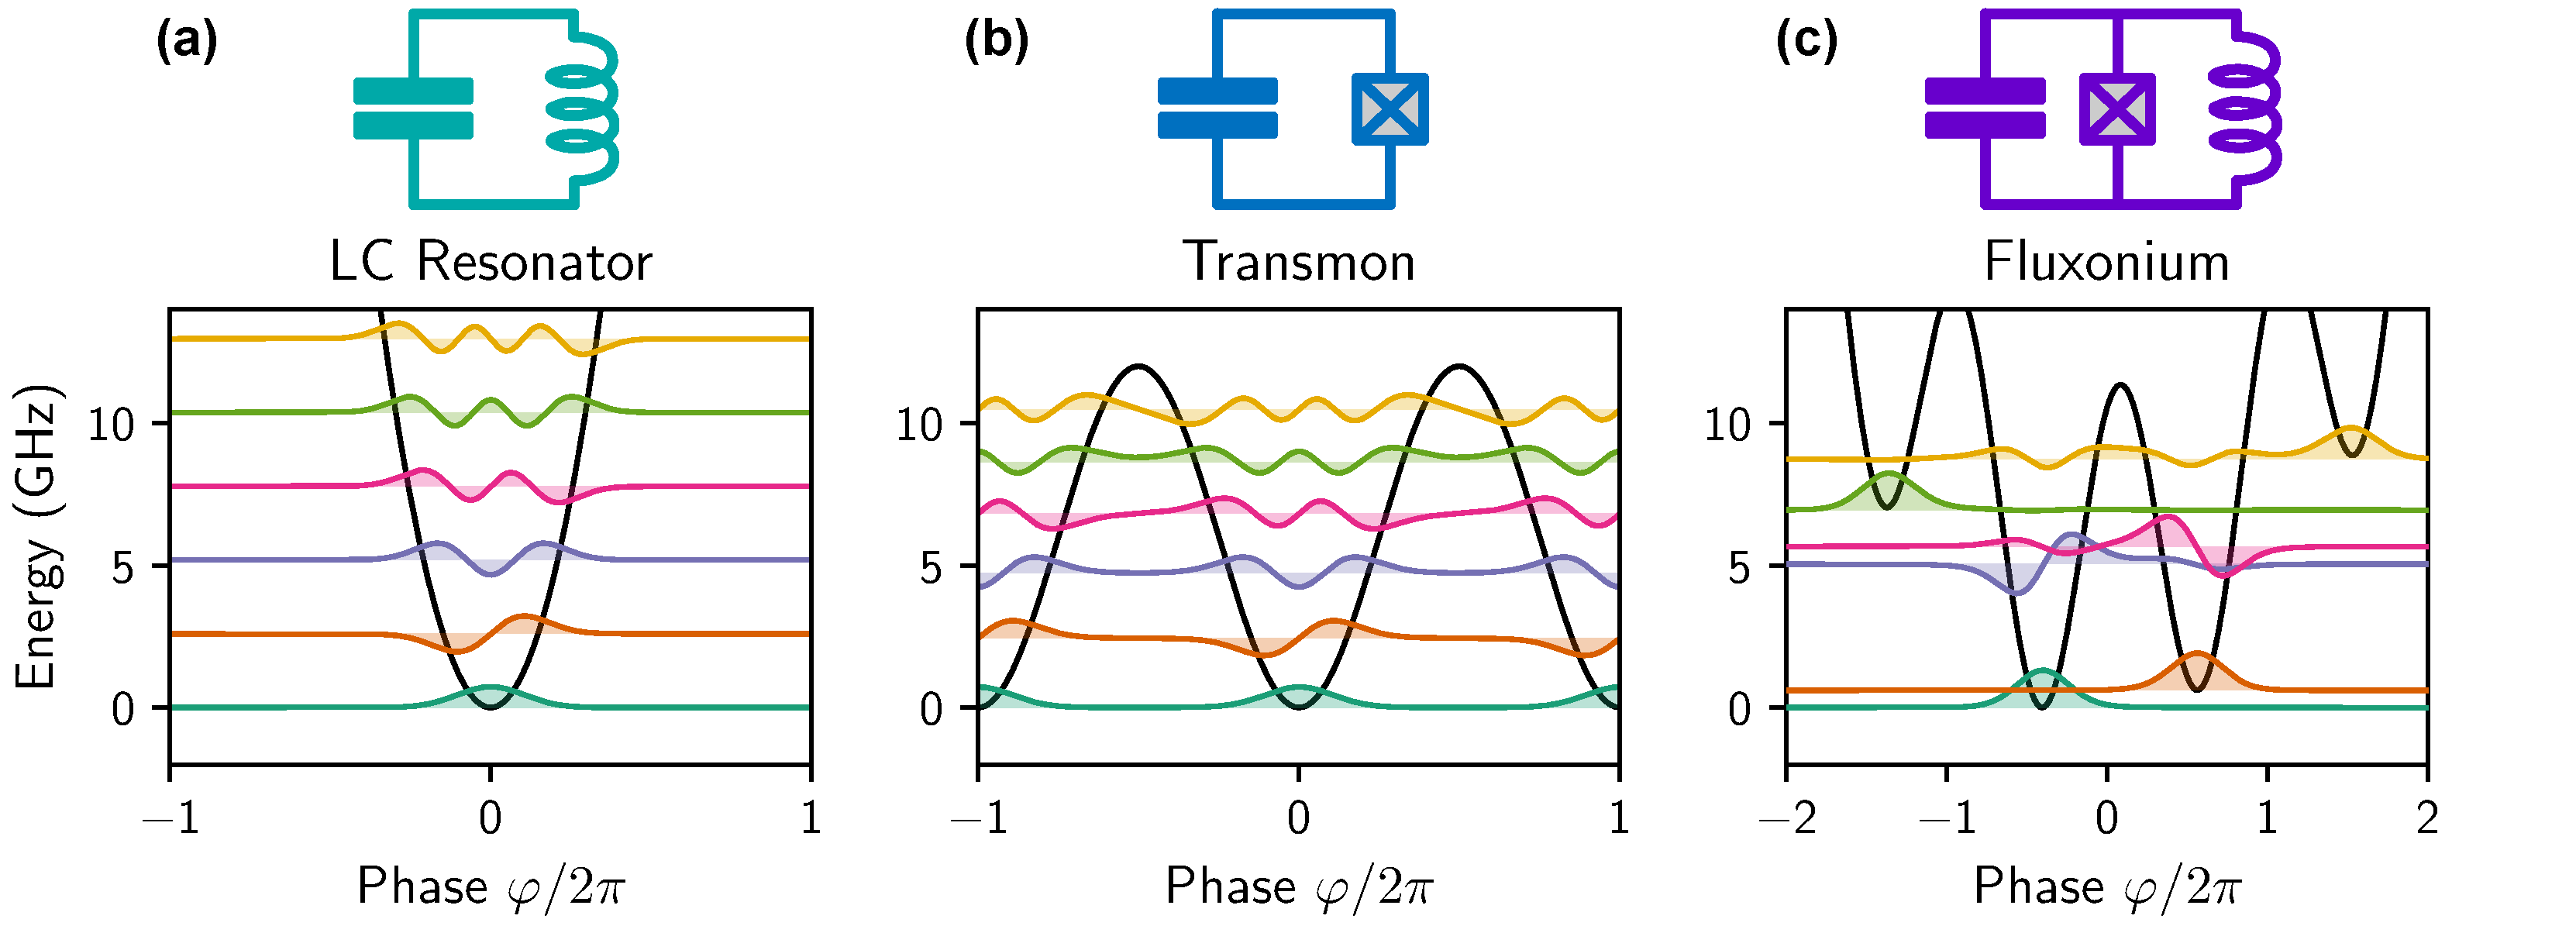
\includegraphics[width=\linewidth]{Figures/3/Circuit_QED_Overview.pdf}
    \caption{The LC resonator, transmon, and fluxonium. We show the circuit diagram, potential, and wavefunctions for each of the three common superconducting circuits.}
    \label{fig:3_Circuit_QED_Overview}
\end{figure}
\clearpage

\section{The LC Resonator}

As its name suggests, an LC circuit consists of a capacitor with capacitance $C$ and inductor with inductance $L$ in parallel. Following Ref. \cite{krantz2019quantum}, we can write a classical Hamiltonian for the LC circuit in terms of the voltage $V(t)$ across the capacitor and the current $I(t)$ flowing through the inductor. These two circuit elements have energies $\frac{1}{2}CV^2$ and $\frac{1}{2}LI^2$ respectively, and thus
\begin{equation}
    H = \frac{1}{2}CV^2 + \frac{1}{2}LI^2
\end{equation}
This Hamiltonian is reminiscent of that of the harmonic oscillator, which we studied in detail in Ch. \ref{ch:2_QEC}. Indeed, if we look at the classical response of this circuit, we find that it behaves like a resonator with resonance frequency $\omega = 1/\sqrt{LC}$. The classical Hamiltonian above can equivalently be written in terms of the charge $Q(t) = CV(t)$ and the flux through the inductive loop $\Phi(t) = LI(t)$. Following \cite{devoret1995quantum}, it will be most convenient to work in terms of these variables so that:
\begin{equation}
    H = \frac{Q^2}{2C} + \frac{\Phi^2}{2L}
\end{equation}
Under this canonical representation, we can think of the flux variable $\Phi$ as a position-like variable of a harmonic oscillator, with the charge variable $Q$ representing the generalized conjugate momentum. We now perform \textit{circuit quantization}, promoting these variables to quantum mechanical operators: $\Phi \to \hat{\Phi}$ and $Q \to \hat{Q}$. We can therefore write the \textit{quantum} Hamiltonian as
\begin{equation}
    \hat{H} = \frac{\hat{Q}^2}{2C} + \frac{\hat{\Phi}^2}{2L} = 4E_C \hat{n}^2 + \frac{1}{2}E_L \hat{\varphi}^2
\end{equation}
where in the second step we define the reduced charge operator $\hat{n} = \hat{Q}/2e$ and reduced phase operator $\hat{\varphi} = 2\pi \hat{\Phi}/\Phi_0$ where $e$ is the electron charge, $\Phi_0 = h/2e$ is the magnetic flux quantum, and we have also defined the charging and inductive energies $E_C = e^2/2C$ and $E_L = (\Phi_0/2\pi)^2/L$ respectively. The operators $\hat{\Phi}$ and $\hat{\Phi}$ are conjugate variables satisfying the canonical commutation relation $[\hat{\Phi}, \hat{Q}] = i\h$, and we can easily check that $[\hat{\varphi}, \hat{n}] = i\h$ as well. Continuing with the association to generalized oscillators, we refer to the inductive term as the potential energy, and the charge term as a kinetic energy. As it will be useful later, we can also define the characteristic \textit{impedance} $Z = \sqrt{L/C}$

As a final step, we can introduce \textit{mode} operators $\hat{a}, \hat{a}^\dagger$ just as we did in Ch. \ref{ch:2_QEC}. We define the transformation
\begin{equation}
    \hat{\varphi} = \varphi_{\rm zpf}(\hat{a} + \hat{a}^\dagger), \quad \hat{n} = in_{\rm zpf}(\hat{a}^\dagger - \hat{a})
\end{equation}
in terms of the zero-point fluctuations $\varphi_{\rm zpf} = (2E_C/E_L)^{1/4}$ and $n_{\rm zpf} =  [E_L/(32E_C)]^{1/4}$ so as to rewrite the Hamiltonian as
\begin{equation}
    \hat{H} = \h\omega\bigg(\hat{a}^\dagger\hat{a} + \frac{1}{2}\bigg)
    \label{eq:3_LC_QHO}
\end{equation}
where $\omega = \sqrt{8 E_LE_C}$. As before, we typically drop the constant term $\h\omega/2$ and sometimes will set $\h\to 1$ in theory derivations, so that $\hat{H} = \omega\hat{a}^\dagger\hat{a}$. We can now use the intuition we developed in Ch. \ref{ch:2_QEC}, and in particular conclude that the LC resonator has Fock states $\ket{n}$ with energy levels $E_n = \h\omega(n+1/2)$. We plot the phase wavefunctions $\psi_n(\varphi)$ associated with these states in Fig. \ref{fig:3_Circuit_QED_Overview} using the parameters $E_C/h = 0.14$ GHz and $E_L/h = 6$ GHz. 

To give some context, superconducting LC circuits are typically operated at microwave frequencies of 1-10 GHz, and are cooled down to ambient temperatures of $T \simeq 20$ mK via a dilution refrigerator. In this limit, we have $k_BT \ll \h\omega$ and thus do not expect significant thermal population of the resonator states. 

To control the LC oscillator, we typically use an external \textit{classical} voltage bias $V_b(t)$ that couples to the circuit via its charge operator; physically, this is realized by some drive line or port that is capacitively coupled. In this case, the driven Hamiltonian can be written as follows:
\begin{equation}
    \hat{H}(t) = \frac{\hat{Q}^2}{2C} + \frac{\hat{\Phi}^2}{2L} + \hat{Q}V_b(t) = \h\omega\hat{a}^\dagger\hat{a} + i\Omega(t) (\hat{a}^\dagger - \hat{a})
\end{equation}
where $\Omega(t) = 2eV_b(t)n_{\rm zpf}$ is typically assumed to have the form $\Omega(t) = \Omega_0\cos(\omega_d t)$ in terms of a drive frequency $\omega_d$ and amplitude $\Omega_0$. As we saw in Sec. \ref{sec:2_control_nonlinearity_drive}, such a classical drive can only produce coherent states in the oscillator. Put equivalently, the resonator energies $E_n$ are all equidistant (with spacing $\h\omega)$, and thus there is no uniquely addressable transition frequency that we can use to create a two-level system (i.e. qubit) from. Therefore, if we want to create a superconducting qubit, we need to introduce some form of \textit{nonlinearity} to the system. 


\section{The Transmon Qubit}

\subsection{Nonlinearity and the Josephson Junction}

We have seen that nonlinearity is a necessary feature for building superconducting qubits. In circuit QED, there is only one circuit element that is both nonlinear and non-dissipative at arbitrarily low temperatures: the Josephson junction, also known as a superconducting tunnel junction \cite{devoret2004superconducting}. Josephson junctions are comprised of two pieces of superconducting metal separated by an insulating layer that is thin enough to allow discrete charges of the superconductor (i.e. Cooper pairs) to tunnel through the barrier. Typically,  junctions are fabricated using aluminium as the superconductor and aluminium oxide as the insulating barrier. The theory behind the Josephson junction is intimately tied to the Bardeen–Cooper–Schrieffer (BCS) theory of superconductivity. While we will not delve into these details here, I recommend the classic text \textit{Introduction to Superconductivity} by Tinkham for a discussion of this \cite{tinkham2004introduction}. Practically, the Josephson junction as a circuit element can be thought of as a nonlinear inductor. It satisfies a current-phase relationship defined by the Josephson equations:
\begin{equation}
    I = I_c \sin(\varphi), \, V = \frac{\h}{2e}\frac{d\varphi}{dt}
    \label{eq:3_josephson_eqs}
\end{equation}
Here $I_c$ is the so-called \textit{critical current} of the junction (i.e. the maximum supercurrent it can support) and $\varphi$ is a variable known as the gauge-invariant phase difference \cite{devoret2021does}, which when quantized can be associated with the reduced phase operator $\hat{\varphi}$. Using Eq. \eqref{eq:3_josephson_eqs}, we find that the inductive potential energy $U(\varphi)$ associated with the Josephson junction is $U(\varphi) = -E_J\cos(\varphi)$ with the so-called \textit{Josephson energy} $E_J$ defined as $E_J = I_c\Phi_0/2\pi$. There is also a finite capacitance $C_J$ associated with a junction, which will give rise to a kinetic energy term $4E_C\hat{n}^2$ in the quantum Hamiltonian\footnote{This is also the Hamiltonian of an older qubit known as the Cooper-Pair Box (CPB) which consisted of just a junction and an external voltage bias. The bias gives rise to an offset voltage or \textit{gate charge} $n_g$ which enters the Hamiltonian via $\hat{H} = 4E_C(\hat{n}-n_g)^2 - E_J\cos(\hat{\varphi})$. However, in the so-called transmon regime that we will discuss in the next section, the gate charge $n_g$ can safely be ignored for the static circuit. } of the junction, which is simply given as the total energy $\hat{H} = 4E_C\hat{n}^2 - E_J\cos(\hat{\varphi})$, with $E_C = e^2/2C_J$. 

\subsection{Hamiltonian of the Transmon}

The \textit{transmon} qubit is formed by placing a Josephson junction in parallel with a large shunt capacitance $C_s$. This capacitance can be added to the intinsic capacitance of the junction $C_J$ to get a total $C_\Sigma = C_J + C_s$. The transmon circuit is shown in Fig. \ref{fig:3_Circuit_QED_Overview} and gives rise to the Hamiltonian
\begin{equation}
    \hat{H} = 4E_C\hat{n}^2 - E_J\cos(\hat{\varphi})
    \label{eq:3_transmon_H}
\end{equation}
with $E_C = e^2/2C_\Sigma$. Since the shunt capacitance is large, the transmon is typically operated in the regime $E_J \gg E_C$ [which is implicit in the definition in Eq. \eqref{eq:3_transmon_H}]. We plot the cosine potential and phase-basis wavefunctions for a transmon in Fig. \ref{fig:3_Circuit_QED_Overview}, using the parameters $E_J/h = 6$ GHz and $E_C/h = 0.14$ GHz. 

In the transmon regime, the phase operator $\hat{\varphi}$ satisfies $\Delta\hat{\varphi} = \sqrt{\ev{\hat{\varphi}^2} - \ev{\hat{\varphi}}^2} \ll 1$, i.e. the phase fluctuations are small. Specifically, if we ignore the periodicity of the potential, we find that the wavefunctions in the region $\varphi \in [-\pi, \pi]$ will be well localized near the bottom of the potential well around $\varphi = 0$, at least for the low-lying energy states. In this case, we can Taylor expand the potential energy term as a power series in $\hat{\varphi}$. More rigorously, it is possible to write  
\begin{equation}
    \hat{H} = 4E_C\hat{n} + \frac{1}{2}E_J \hat{\varphi}^2 - E_J\bigg[\cos(\hat{\varphi}) + \frac{1}{2}E_J \hat{\varphi}^2\bigg]
\end{equation}
The first two terms can be expressed in terms of oscillator-like mode operators $\hat{q}, \hat{q}^\dagger$ defined as $\hat{\varphi} = \varphi_{\rm zpf}(\hat{q} + \hat{q}^\dagger)$ and $\hat{n} = in_{\rm zpf}(\hat{q}^\dagger - \hat{q})$ with $\varphi_{\rm zpf} = (2E_C/E_J)^{1/4}$ and $n_{\rm zpf} =  [E_J/(32E_C)]^{1/4}$. In the transmon regime, $\varphi_{\rm zpf} \ll 1$ and so we can expand the remaining nonlinear term. To leading order, 
\begin{equation}
    \hat{H} \approx 4E_C\hat{n}^2 + \frac{1}{2}E_J \hat{\varphi}^2 - \frac{E_J}{24}\hat{\varphi}^4 = \omega_q \hat{q}^\dagger \hat{q} - \frac{E_C}{12}(\hat{q} + \hat{q}^\dagger)^4
    \label{eq:transmon_duffing_H}
\end{equation}
where $\omega_q = \sqrt{8 E_C E_J}$. When written this way, it is immediately evident that the transmon is essentially a nonlinear oscillator. Using perturbation theory, we find that the energies are approximately \cite{bishop2010circuit}:
\begin{equation}
    E_m \simeq m\omega_q - \frac{E_C}{12}\big[6m^2 + 6m\big]
\end{equation}
which, as desired for a qubit, are nonlinear in $m$. To get to this, we can expand the quartic nonlinearity and, after normal ordering, keep only the number-conserving terms $\hat{q}^\dagger{}^n\hat{q}^n$, which is tantamount to performing a rotating-wave approximation. Doing so, we get the simplified Hamiltonian
\begin{equation}
    \hat{H} = [\omega_q + \alpha]\hat{q}^\dagger \hat{q} + \frac{\alpha}{2}\hat{q}^\dagger{}^2\hat{q}^2
\end{equation}
where we have defined the \textit{anharmonicity} as $\alpha = -E_C$, and we refer to $\omega_{\rm ge} = \omega_q + \alpha$ as the qubit transition frequency. Since the $\ket{g}\to\ket{e}$ and $\ket{e}\to\ket{f}$ transitions are now detuned from each other by $\alpha = \omega_{ef}-\omega_{ge}$, we can treat the lowest two levels $\ket{g}$ and $\ket{e}$ as a two-level qubit, for which
\begin{equation}
    \hat{H} \approx \frac{\omega_{\rm ge}}{2}\sigmaz
\end{equation}
Here, we made a two-level approximation $\hat{q} \to \sigmam$, $\hat{q}^\dagger \to \sigmap$ and so $\hat{q}^\dagger \hat{q} \to (1 - \sigmaz)/2$ and we drop the minus sign by convention. Finally, to give perspective, typical transmons have frequencies $\omega_{\rm ge}$ in the range of 4-6 GHz, and anharmonicities $|\alpha|$ around 100-400 MHz. 

\subsection{Coupling a Transmon and a Resonator}

The basis of circuit QED involves coupling superconducting qubits and resonators to form a spin-oscillator model. Thus, let us briefly touch on how we couple a transmon qubit to an LC resonator. We typically use a capacitive coupling model with an interaction of the form $\hat{H}_{\rm int} = J_{aq} \hat{n}_a \hat{n}_q$ with coupling strength $J_{aq}$ between the charge operators of the oscillator and qubit respectively. The total Hamiltonian for the coupled system is given by
\begin{equation}
    \hat{H} = \hat{H}_a + \hat{H}_q + \hat{H}_{\rm int} = \omega_a \hat{a}^\dagger\hat{a} + \Big[4E_C\hat{n}^2 - E_J\cos(\hat{\varphi})\Big] + \hat{H}_{\rm int}
    \label{eq:3_transmon_resonator_full}
\end{equation}
Expressing the transmon in terms of its mode operators and defining $g = -J_{aq}n_{{\rm zpf},a}n_{{\rm zpf},q}$, we have 
\begin{equation}
    \hat{H} = \omega_a \hat{a}^\dagger\hat{a} + \omega_{\rm ge}\hat{q}^\dagger \hat{q} + \frac{\alpha}{2}\hat{q}^\dagger{}^2\hat{q}^2 + g(\hat{a}-\hat{a}^\dagger)(\hat{q}-\hat{q}^\dagger)
    \label{eq:3_transmon_resonator_linear_coupling}
\end{equation}
with a bilinear coupling in $\hat{a}$ and $\hat{q}$. At this point, we can truncate to a two-level qubit and perform a rotating-wave approximation (RWA) on the coupling term, which is standard in the literature \cite{blais2021circuit}. Doing so will give us a Jaynes-Cummings type Hamiltonian as we saw in Sec. \ref{sec:2_control_nonlinearity_drive}:
\begin{equation}
    \hat{H} = \omega_a \hat{a}^\dagger\hat{a} + \frac{\omega_{\rm ge}}{2}\sigmaz + \big[\hat{a}^\dagger\sigmam + \hat{a}\sigmap\big]
    \label{eq:3_JC_Hamiltonian_transmon}
\end{equation}
As we did there, we can further transform this Hamiltonian to a dispersive coupling model in the limit $g \ll |\omega_a - \omega_{\rm ge}|$. For a truly two-level system starting from Eq. \eqref{eq:3_JC_Hamiltonian_transmon}, this gives the Hamiltonian
\begin{equation}
    \hat{H}_{\rm disp} = \omega_a' \hat{a}^\dagger\hat{a} + \frac{\omega_{\rm ge}'}{2}\sigmaz + \frac{\chi}{2}\hat{a}^\dagger\hat{a}\sigmaz
    \label{eq:3_dispersive_model_transmon_TLS}
\end{equation}
with the definitions $\chi = 2g^2/\Delta$, $\omega_a' = \omega_a$, and $\omega_{\rm ge}' = \omega_{\rm ge} + g^2/\Delta$ in terms of $\Delta = \omega_{\rm ge} - \omega_a$. As we previously saw, this dispersive Hamiltonian forms the basis of most of modern circuit QED and also gives a blueprint for qubit readout, since we can determine the qubit state by measuring the effective frequency $\omega_a' + \chi \hat{a}^\dagger\hat{a}\ev{\sigmaz}/2$ of the resonator \cite{blais2004cavity}. 

For realistic transmons, it turns out to be not quite correct to truncate to a two-level qubit before making the dispersive approximation. If we instead make the dispersive approximation at the level of Eq. \eqref{eq:3_transmon_resonator_linear_coupling} and \textit{then} truncate, we get a final Hamiltonian with the same form as Eq. \eqref{eq:3_dispersive_model_transmon_TLS} but with redefined $\omega_a' = \omega_a - g^2/(\Delta - E_C/\h)$, $\omega_{\rm ge}' = \omega_{\rm ge} + g^2/\Delta$, and $\chi = - (g^2E_C/\h) / [\Delta(\Delta - E_C/\h)]$. 

\noindent\textbf{Black-Box Quantization.} There is another way to treat a coupled transmon and resonator that makes use of the oscillator-like character of the transmon \cite{nigg2012black}. Starting from the full model in Eq. \eqref{eq:3_transmon_resonator_full} and performing the RWA on the coupling, we can write the Hamiltonian as:
\begin{equation}
    \hat{H} = \omega_a \hat{a}^\dagger\hat{a} + \omega_q \hat{q}^\dagger\hat{q} + g\big[\hat{a}^\dagger\hat{q} + \hat{a}\hat{q}^\dagger\big] - E_J\bigg[\cos(\hat{\varphi}) + \frac{1}{2}E_J \hat{\varphi}^2\bigg]
\end{equation}
The first three terms describe two linearly coupled oscillators which can be diagonalized exactly to get two normal modes $\hat{a}'$ (oscillator-like) and $\hat{q}'$ (qubit-like) with frequencies $\omega_a'$ and $\omega_q'$. The phase of the transmon $\hat{\varphi} = \varphi_{\rm zpf}(\hat{q} + \hat{q}^\dagger)$ can then be expressed as a superposition of the new modes $\hat{\varphi} = \varphi_a(\hat{a}' + \hat{a}'{}^\dagger) + \varphi_q(\hat{q}' + \hat{q}'{}^\dagger)$ with \textit{participation ratios} $\varphi_a$, $\varphi_q$. At this point, we can now truncate the nonlinear potential term of the transmon and keep just the quartic term $-E_J\hat{\varphi}^4/24$. For brevity, but at the risk of confusion, I now drop the $'$ and write
\begin{equation}
    \hat{H} = \omega_a \hat{a}^\dagger\hat{a} + \omega_q \hat{q}^\dagger\hat{q} - \frac{E_J}{24}\big[\varphi_{a}(\hat{a} + \hat{a}^\dagger) + \varphi_{q}(\hat{q} + \hat{q}^\dagger)\big]^4
\end{equation}
\textit{in the normal mode basis} (this is important to keep in mind; we really mean $\hat{a}'$ and $\hat{q}'$ above). From here, we can expand the quartic term to get various monomials. Again invoking the RWA, we keep only the number-conserving terms in the expansion. This gives an effective Hamiltonian:
\begin{equation}
    \hat{H} = \omega_a \hat{a}^\dagger\hat{a} + \omega_q \hat{q}^\dagger\hat{q} + \frac{\chi_{aq}}{2}\hat{a}^\dagger\hat{a}\hat{q}^\dagger\hat{q}  + \frac{K_a}{2}\hat{a}^\dagger{}^2\hat{a}^2 + \frac{K_q}{2}\hat{q}^\dagger{}^2\hat{q}^2
\end{equation}
where we now have a dispersive shift $\chi_{aq} \triangleq -E_J\varphi_a^2 \varphi_q^2/2$ and so-called \textit{Kerr} nonlinearities $K_q \triangleq -E_J\varphi_q^4/4$ and $K_a \triangleq -E_J\varphi_a^4/4$ for the qubit and oscillator, with the former just being the qubit's anharmonicity. This Hamiltonian is similar to Eq. \ref{eq:3_dispersive_model_transmon_TLS} in that it has a dispersive coupling, but differs in that the oscillator now inherits some nonlinearity as well. This can be particularly harmful when we are trying to use oscillators for bosonic QEC (e.g. with a GKP code), since bosonic codes typically assume a linear oscillator mode. 


% \vfill
% \begin{greybox}
%     \textbf{Generalization of black-box quantization:} We use the black-box quantization (BBQ) approach extensively in our research 
% \end{greybox}
% \todo{} Maybe mention how we have generalized BBQ?

\clearpage
\section{The Fluxonium Qubit}

We are now ready to discuss the main qubit of interest for this thesis: the fluxonium \cite{manucharyan2009fluxonium}. A fluxonium consists of a linear inductor, a capacitor, and a Josephson junction in parallel, with energies $E_L$, $E_C$, and $E_J$ respectively. A corresponding circuit diagram for this qubit is shown in Fig. \eqref{fig:3_Circuit_QED_Overview}. While it may be tempting to simply add together the various energy terms that we have seen previously, there is one additional piece of theoretical background required, known as \textit{flux quantization}. 

Fluxonium is a type of generalized \textit{flux qubit}, and thus it is possible to thread an external magnetic flux $\Phi_{\rm ext}$ through the loop between the junction and the inductor. If we define the branch variables $\Phi_J$ and $\Phi_L$ for these two elements respectively, then the flux quantization condition can be expressed \cite{orlando1991foundations}:
\begin{equation}
    \Phi_J - \Phi_L = \Phi_{\rm ext}
\end{equation}
This is a holonomic constraint on the phase variables; there is thus only one effective phase degree of freedom in the circuit. Working in terms of the reduced variables $\varphi_k = 2\pi \Phi_k/\Phi_0$, we can choose to allocate\footnote{Note that for \textit{time-dependent} external fluxes $\varphi_{\rm ext} = \varphi_{\rm ext}(t)$, the choice of allocation becomes more subtle and it turns out we should instead group the external flux with the inductor $\varphi_L = \varphi - \varphi_{\rm ext}$. After performing circuit quantization, the fluxonium Hamiltonian then reads $\hat{H} = 4E_C \hat{n}^2 + \frac{1}{2}E_L[\hat{\varphi} - \varphi_{\rm ext}]^2 - E_J\cos(\hat{\varphi})$ \cite{you2019circuit}.} the external flux via $\varphi_J = \varphi + \varphi_{\rm ext}$ and $\varphi_L = \varphi$. The inductive energy of the inductor is then $\frac{1}{2}E_L\varphi^2$, while the Josephson energy is $-E_J\cos(\varphi + \varphi_{\rm ext})$. We therefore finally get
\begin{equation}
    \hat{H} = 4E_C \hat{n}^2 + \frac{1}{2}E_L\hat{\varphi}^2 - E_J\cos(\hat{\varphi} + \varphi_{\rm ext})
    \label{eq:3_fluxonium_H}
\end{equation}
for the fluxonium Hamiltonian after circuit quantization. In practice, the inductive energy is $E_L \sim 0.5$ GHz, corresponding to a large inductance $L \sim 325$ nH \cite{nguyen2022blueprint}. There are various approaches to realize such a \textit{superinductance}, such as using granular aluminum \cite{maleeva2018circuit, grunhaupt2019granular, kamenov2020granular, rieger2023granular} or geometric inductances \cite{peruzzo2020surpassing, peruzzo2021geometric}, but by far the most common strategy is to use an array of Josephson junctions \cite{manucharyan2009fluxonium, masluk2012microwave}, as we show in Fig. \ref{fig:3_Superinductance}. A nice pedagogical derivation of how a chain of $N$ Josephson junctions behaves like a linear inductor in the limit of large $N$ can be found in the excellent PhD thesis of EQuS alum Leon Ding \cite{ding2023thesis}. 

\begin{figure}
    \centering
    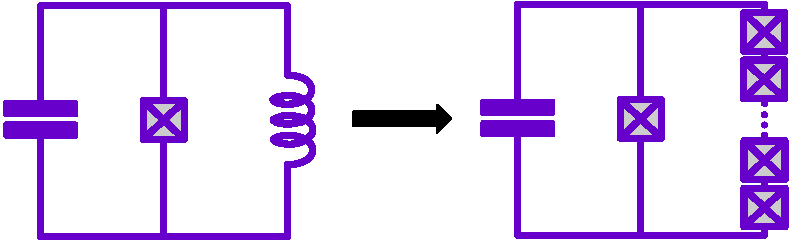
\includegraphics[width=0.7\linewidth]{Figures/3/Superinductance.pdf}
    \caption{The superinductance in a fluxonium is typically implemented via an array of $N$ Josephson junctions, which behave approximately like a linear inductor for large $N$.}
    \label{fig:3_Superinductance}
\end{figure}

As a final remark on the Hamiltonian, we note that the inductive and charging terms of Eq. \eqref{eq:3_fluxonium_H} can be diagonalized using the $E_L$-$E_C$ Fock basis, as done for the LC circuit. This allows us to write
\begin{equation}
    \hat{H} = \omega_q\hat{q}^\dagger\hat{q} - E_J\cos(\hat{\varphi} + \varphi_{\rm ext})
\end{equation}
for the \textit{full} Hamiltonian, with $\omega_q = \sqrt{8 E_LE_C}$ and $\hat{\varphi} = (2E_C/E_L)^{1/4}[\hat{a} + \hat{a}^\dagger]$ as in Eq. \eqref{eq:3_LC_QHO}. Using this basis, it is possible to numerically diagonalize the full fluxonium Hamiltonian. We plot such an example with the phase-basis wavefunctions in Fig. \ref{fig:3_Circuit_QED_Overview}, using parameters $E_J/h = 6$ GHz,  $E_L/h = 0.2$ GHz, $E_C/h = 0.14$ GHz, and $\Phi_{\rm ext} = 0.42\Phi_0$. 

The regime we are interested in for the fluxonium is the so-called heavy regime in which $E_J \gg E_C \approx E_L$. When $\Phi_{\rm ext} = 0.5\Phi_0$, the potential energy has a double-well structure, with the lowest energy states $\ket{g}$ and $\ket{e}$ given by symmetric and antisymmetric combinations of the two wells' localized wavefunctions, and the qubit frequency $\omega_{\rm ge}$ becomes small; the heaviness of a fluxonium can be characterized by the splitting $\omega_{\rm ge}$ at this half-flux point, with typical heavy fluxoniums having qubit frequencies of about 10-300 MHz, with lower $\omega_{\rm ge}$ translating to ``heavier'' \cite{earnest2018realization, zhang2021universal, ding2023FTF}. Meanwhile, if we move slightly off this half-flux point, the ground and excited states will have a larger energy splitting and be strongly localized to their respective wells, as is shown in Fig. \ref{fig:3_Circuit_QED_Overview}. When operated as a low-frequency qubit, the fluxonium has $\omega_{\rm ge} \ll \alpha$ (the anharmonicity), which truly enables us to think of it as a two-level system. Also, the charge matrix element vanishes $\mel{g}{\hat{n}}{e} \to 0$. This in turn has led to heavy fluxonium qubits reporting $T_1$ lifetimes (between states $\ket{g}$ and $\ket{e}$) in excess of 1 ms at the half-flux sweet spot, and typically even larger away from it \cite{earnest2018realization, zhang2021universal, ding2023FTF, nguyen2019high, somoroff2023millisecond}. It is for this reason that we are interested in the fluxonium, as a bit-flip protected control qubit. 

\subsection{Circuit QED with the Fluxonium}

Just as we did for the transmon, let's now briefly examine how to couple a fluxonium to a harmonic oscillator. The basic model we follow is that of Ref. \cite{zhu2013cQEDfluxonium}, which starts from the Hamiltonian
\begin{equation}
    \hat{H} = \sum_k \omega_k \op{k}{k} + \omega_a \hat{a}^\dagger\hat{a} + g\hat{n}(\hat{a} + \hat{a}^\dagger)
\end{equation}
in terms of the bare fluxonium eigenstates $\ket{k}$ and coupling strength $g$. When we deal with this Hamiltonian in practice, we will typically just numerically diagonalize and calculate the hybridized energy levels $E_{k, n}$ associated with a qubit state $k$ and resonator state $n$; to be more precise, we diagonalize the coupled system to get eigenenergies $\epsilon_i$ and eigenstates $\ket{v_i}$ and then perform \textit{quantum number assignment} to label each state in terms of the uncoupled basis state $\ket{k}\otimes\ket{n}$ that it is closest to (i.e. largest overlap). In this manner, we can get the \textit{labelled} energies $E_{k, n}$ and eigenstates $\ket{k, n}$ for the hybridized system. 








\begin{equation}
    \hat{H} = \sum_k \tilde{E}_k \op{k}{k} + \bigg(\omega_r^0 + \sum_k \chi_k \op{k}{k}\bigg) \hat{a}^\dagger\hat{a}
\end{equation}



write down equation from MM talk depending on flux... 